%!TEX encoding = IsoLatin

%\chapter{Architecture logique}

\section{Diagramme de package}

\begin{figure}[H]
	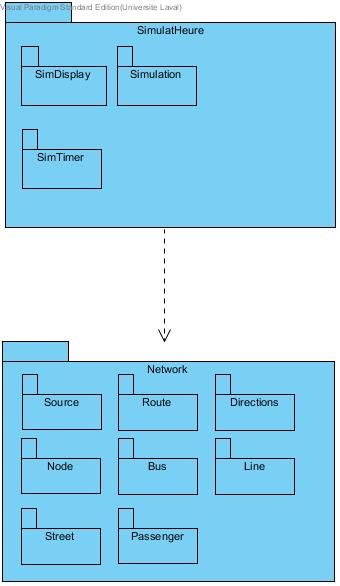
\includegraphics[scale=0.5]{fig/packageDiagram.jpg}
	\centering
	\caption{Diagramme de package de SimulatHEURE}
	\label{f:package_Diag}
\end{figure}

\paragraph{}
La figure \ref{f:package_Diag} pr�sente la structure logique des modules du programme. Le module principal, nomm� SimulatHeure, est compos� des classes SimDisplay et SimTimer et Simulation, dont le fonctionnement est expliqu� au paragraphe suivant. Le Module SimulatHeure appelle et contr�le un second module g�rant le fonctionnement du r�seau routier, d'o� son nom "Network". Ce dernier est constitu� de tout les �l�ments composant un r�seau d'autobus, incluant \textit{Node}, \textit{Line}, \textit{Source}, \textit{Directions}, \textit{Route}, \textit{Bus} et \textit{Passenger}. L'interaction des classes dans Network est pr�sent� en d�tail plus loin.
\paragraph{}
La classe \textit{Simulation} est le cerveau de la simulation. C'est elle qui contient les listes des diff�rentes composantes du r�seau routier. Elle permet d'ajouter, de supprimer et de faire bouger les diff�rentes composantes du r�seau routier. La classe \textit{SimDisplay}, incorpor�e dans le module SimulatHeure, prend en charge l'affichage en temps r�el de la simulation des transports. Son champs d'actions couvre entre autres le dessin des �l�ments du r�seau sur la fen�tre de simulation, la gestion des contr�les usagers avec la souris (d�placement de la vue, zoom, dezoom, selection, etc.) ainsi que l'affichage de la grille d'alignement dynamique. La classe \textit{SimTimer} permet d'appeller p�riodiquement la fonction simulateTick() de \textit{Simulation}, ce qui met en marche la simulation.
\paragraph{}
Les classes dans \textit{Network} sont toutes des classes purement logique, c'est � dire qu'elle n'ont aucun lien avec l'interface utilisateur. Les divers �l�ments tels les noeuds, les segments o� les bus poss�dent des attributs spatiaux, correspondant � leur position sur une grille virtuelle, qui doit �tre configur�e de fa�on externe, ici par un contr�lleur et un panneau d'affichage graphique.  C'est le contr�lleur qui permet de faire int�ragir les diff�rentes classes ensemble par leurs fonctions.

